\documentclass[10pt,border=1pt]{standalone}
\usepackage[T1]{fontenc}
\usepackage{mathptmx}
\usepackage{amsmath,amssymb}
\usepackage[table]{xcolor}
\usepackage{tikz}
\usetikzlibrary{positioning,arrows.meta,calc,fit,decorations.pathreplacing}
\definecolor{fmblue}{HTML}{2A78D6}
\definecolor{cnnorange}{HTML}{EB6834}
\definecolor{inkgray}{HTML}{52514E}
\definecolor{lightfill}{HTML}{F1F0EC}
\tikzset{
  arr/.style={-{Stealth[length=2.2mm]}, draw=inkgray, line width=0.7pt},
  blk/.style={draw=inkgray, rounded corners=2pt, fill=white, align=center, inner sep=3pt, font=\fontsize{10}{12}\selectfont},
  frz/.style={blk, fill=lightfill},
  trn/.style={blk, fill=fmblue!14},
  trn2/.style={blk, fill=cnnorange!16},
  note/.style={align=left, font=\fontsize{10}{12}\selectfont\itshape, text=inkgray},
}
\begin{document}
\fontsize{10}{12}\selectfont

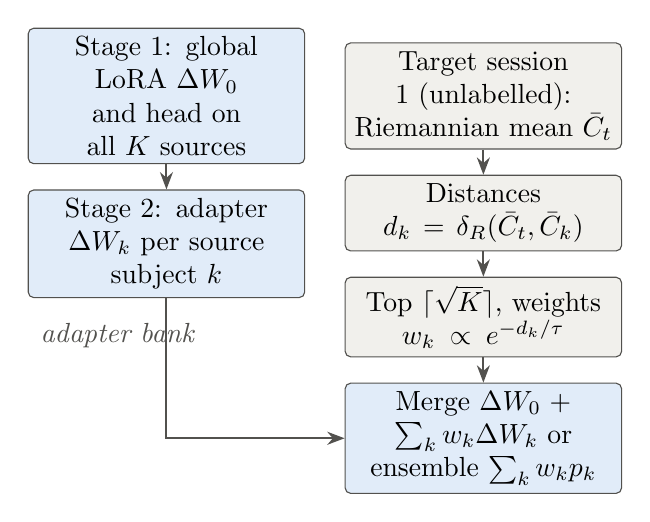
\begin{tikzpicture}[node distance=0.32cm]
\node[trn, text width=3.3cm] (s1) {Stage 1: global LoRA $\Delta W_0$ and head on all $K$ sources};
\node[trn, text width=3.3cm, below=of s1] (s2) {Stage 2: adapter $\Delta W_k$ per source subject $k$};
\node[frz, text width=3.3cm, right=0.5cm of s1] (tm) {Target session 1 (unlabelled): Riemannian mean $\bar C_t$};
\node[frz, text width=3.3cm, below=of tm] (d) {Distances $d_k=\delta_R(\bar C_t,\bar C_k)$};
\node[frz, text width=3.3cm, below=of d] (w) {Top $\lceil\sqrt K\rceil$, weights $w_k\propto e^{-d_k/\tau}$};
\node[trn, text width=3.3cm, below=of w] (m) {Merge $\Delta W_0+\sum_k w_k\Delta W_k$ or ensemble $\sum_k w_k p_k$};
\draw[arr] (s1)--(s2); \draw[arr] (tm)--(d); \draw[arr] (d)--(w); \draw[arr] (w)--(m);
\draw[arr] (s2.south) |- (m.west);
\node[note, below=0.2cm of s2, text width=3.2cm] {adapter bank};
\end{tikzpicture}
\end{document}
